\chapter{Praktischer Teil}

Im Folgenden werden die verschiedene praktische Lösungsansätze vorgestellt und anhand verschiedener Kriterien gegeneinander abgewogen, sodass am Ende eine Handlungsmatrix erstellt werden kann.

\section{Lösungsansätze}

Zunächst sollen drei verschiedene Technologien vorgestellt werden, mit denen sich asynchrone Prozesse mit sequentieller Kommunikation, trotz den Einschränkungen durch RAP und Fiori Elements, umsetzen lassen.

\subsection{Business Workflows}

Der erste mögliche Ansatz sind Business Workflows (BW abgekürzt). BWs können benutzt werden um jeglichen Geschäftsprozess im SAP-System abzubilden. Sie decken das Spektrum von einfachen Genehmigungsprozessen bis hin zu komplexen Abläufen ab. Sie eignen sich vor allem für repetitive Prozesse mit mehreren Bearbeitern. BWs können zudem zur Fehlerbehandlung in anderen Prozessen oder eventgesteuert eingesetzt werden. Mit Workflows können durch die Benutzung der bereits bestehenden Funktionen und Transaktionen des SAP-Systems neue Geschäftsprozesse abgebildet werden. Die Funktionen und Transaktionen an sich werden dabei durch den Workflow nicht verändert. In Kombination mit Organisationsmanagement können die einzelnen Schritte des BW durch bestimmte Akteure ausgeführt werden. Das kann auch auf bestimmte Stellen abstrahiert werden, um von personellen Veränderungen innerhalb des Unternehmens unabhängig zu sein. Workflows können auch untereinander durch das Versenden und Konsumieren von Nachrichten kommunizieren. Diese Kommunikation ist auch zwischen verschiedenen SAP-Systemen über das Internet mit XML-Dokumenten möglich. \footcite[Vgl.][]{sap_business-workflows_2022-1}

\subsubsection{Aufbau eines Business Workflows}

Zunächst wird die Definition der Aufbau eines Business Workflows beschrieben. Diese lässt sich in vier Bereiche unterteilen.

\begin{figure}[H]
 \centering
 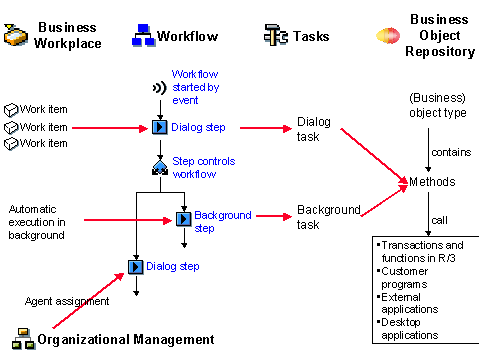
\includegraphics[height=8cm]{Bilder/Business-Workflows_Schema.png}
 \caption[Aufbau eines Business Workflows]{Aufbau eines Business Workflows, Abgerufen von \cite{sap_business-workflows_2022-1} am 17.07.2023.}
 \label{fig:iso_norm}
\end{figure}

Der Business Workplace ist der Ort in einem SAP-System, in dem der Endanwender ''work items'' (übersetzt aus dem Englischen: ''Arbeitspakete'' oder ''Aufgaben'') abhängig vom Zeitpunkt im Geschäftsprozess und den Berechtigungen des Users ausführen kann. Ein work item stellt zur Laufzeit des BW einen Schritt des Prozesses dar, der ausgeführt wird. Es werden hier jedoch nicht alle work items angezeigt. So werden \zB solche, die einem Prozess-Schritt, der im Hintergrund ausgeführt werden soll, zugeordnet sind, hier nicht angezeigt. \footcite[Vgl.][]{sap_business-workflows_2022-1}

Ein Workflow muss vor Ausführung in der ''workflow definition'' angelegt werden. Diese Definition legt die Reihenfolge der auszuführenden Schritte des Prozesses fest und enthält zudem Kontrollschritte. Zusätzlich können noch Bearbeiter und Fristen für bestimmte Schritte festgelegt werden, die dann zur Laufzeit des Workflows vom ''Work item manager'' verwaltet werden. Es gibt viele Arten von Schritten, die gängigen Konzepten in der Programmierung ähneln, wie \zB normale Aktivitäten, Fallunterscheidungen, Schleifen. Zudem gibt es Schritte zum Versenden von Nachrichten, Auslösen von Events, Benutzerentscheidungen, usw. Diese Schritte können entweder im Dialog mit einem Benutzer ausgeführt werden, wenn \zB die Eingabe bestimmter Werte erforderlich ist, oder automatisch vom System im Hintergrund ausgeführt werden. Ein Workflow kann nicht nur manuell von einem Benutzer gestartet werden, sondern auch systemseitig von einem bestimmten Event ausgelöst werden. Hierfür muss in der Definition des Workflows das gewünschte Event als Auslöser angegeben werden. Wenn dann das Event auftritt, wird der Workflow automatisch gestartet. Im betrieblichen Kontext könnte hier \zB ein Mitarbeiter einen Urlaubsantrag stellen, der dann den als Workflow abgebildeten Genehmigungsprozess auslöst. Das wäre ein Beispiel für einen asynchronen Prozess mit sequentieller Kommunikation. \footcite[Vgl.][]{sap_business-workflows_2022-1}

Die einzelnen Schritte, die innerhalb des Workflows ausgeführt werden, hei{\ss}en Tasks und stellen grundlegende betriebliche Tätigkeiten dar. Die Dialog- und Hintergrund-Schritte in der Workflow Definition korrespondieren hier mit Dialog- oder Hintergrund-Tasks. Im Workflow bezieht sich ein Task immer auf eine Methode eines Objekttyps. Diese Methoden können automatisch ausführbar sein oder müssen aktiv von einem Benutzer gestartet werden. Eine Methode kann einerseits Transaktionen oder Funktionen innerhalb des ERP-Systems aufrufen. Spezielle Anforderungen können durch kundeneigene Logik, oder Schnittstellen zu anderen Systemen umgesetzt werden. \footcite[Vgl.][]{sap_business-workflows_2022-1}

Methoden, die innerhalb eines Workflows aufgerufen werden, sind immer Teil von Objekten. Diese Objekte können auch BOs sein. Im Allgemeinen ist ein Objekt ein konkreter Datensatz eines Objekttyps. Die Daten des Objekts werden durch seine Attribute definiert und die Aktionen, wie das Erstellen, Aktualisieren oder Löschen von Daten wird durch die Methoden des Objekts beschrieben. Einen weiteren wichtigen Teil von Objekten stellen Events dar. Diese werden ausgelöst, wenn bei einem Objekt seinen Status verändert. Das kann \zB durch das Erstellen, Verändern oder Löschen von Daten passieren. Diese Events können dann unter anderem Workflows starten. Das ''Business Object Repository'' bietet eine Übersicht über alle in einem SAP-System verfügbaren Objekttypen. Man kann die bereits vorhandenen Objekttypen bei Bedarf anpassen oder neue erstellen. \footcite[Vgl.][]{sap_business-workflows_2022-1}

\subsection{Business Events}

Der zweite Ansatz ist die Umsetzung mit Business Events (BE abgekürzt). Business Events sind Events die von BOs erzeugt und konsumiert werden können. Dieser eventgesteuerte Kommunikationsansatz, der die asynchrone Kommunikation zwischen dem Event-erzeugenden und -konsumierenden BO ermöglicht, wird von RAP im Standard unterstützt. Hier ist keine direkte Antwort des Empfängers nötig, ein BO erzeugt ein Event und dieses wird von anderen BOs dann weiterverarbeitet, ohne dass der Erzeuger weiterhin in diesen Prozess involviert ist Somit spricht man hier von einer einseitigen, also asynchronen Kommunikation. 
Ein BE stellt eine signifikante Veränderung eines BO dar, die im Zuge eines Behaviours erzeugt wird. Dem Event werden dann über dessen Metadaten alle nötigen Informationen, anhand derer die Weiterverarbeitung, je nach speziellem Anwendungsfall, stattfindet, mitgegeben. \footcite[Vgl.][]{sap_business-events_2023}

Ein BO kann als Event-Erzeuger oder Event-Konsument auftreten. Zuerst wird die Erzeuger-Seite betrachtet.

\begin{figure}[H]
 \centering
 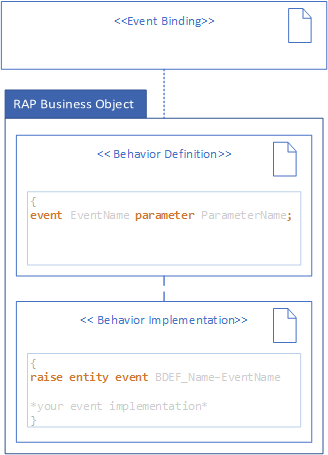
\includegraphics[height=8cm]{Bilder/Business-Events_BO-as-event-consumer.png}
 \caption[Business Object als Event-Erzeuger]{Business Object als Event-Erzeuger, Abgerufen von \cite{sap_business-events_2023} am 17.07.2023.}
 \label{fig:iso_norm}
\end{figure}

Ein Event wird in der Behaviour Definition eines BO erstmals definiert. Hier können dann Parameter für die weitere Verarbeitung mitgegeben werden, die dann in den Metadaten des Events mitgeschickt werden. Danach kann es in der dazugehörigen Behaviour Implementation innerhalb einer speziellen Operation des BO erzeugt werden. Ein Event wird zu dem Zeitpunkt in RAP Laufzeit erzeugt, nachdem die Veränderungen des BO, die das Event auslösen, auf der Datenbank persistiert wurden. Durch das Event Binding wird das Event noch einem speziellen Namensraum, BO und zugehöriger Operation zugeordnet. \footcite[Vgl.][]{sap_business-events_2023}

BOs können BEs nicht nur erzeugen, sondern auch verarbeiten. Dies geschieht über das Event Consumption Model. Ein Event Consumption Model besteht aus einer Reihe von ABAP-Artefakten, mit denen man Events im SAP-System konsumieren kann. Diese Events müssen jedoch dem Standard eines Cloud Events entsprechen, da der Austausch über das SAP Event Mesh abgewickelt wird, was ein Dienst der SAP Business Technology Platform und somit komplett cloud-basiert ist. Hierfür muss ein inbound bzw. outbound Event-Binding für ein- bzw. ausgehende Events erstellt werden. Diese Bindings sind Teil des SAP Enterprise Event Enablement Frameworks, das den Austausch von Events zwischen dem S/4 System und der BTP regelt. \footcite[Vgl.][]{sap_creating_2022}

\subsection{Background Processing Framework}

Die letzte Möglichkeit, die betrachtet wird, um asynchrone Prozesse abzubilden, stellt das ''background Processing Framework'' (bgPF abgekürzt) dar.

Das bgPF ist ein Framework, das die Möglichkeit schafft asynchron zum Hauptprozess Logik auszulagern und auszuführen. Zuerst soll auf die grundlegende Funktionsweise des bgPF eingegangen werden.

\begin{figure}[H]
 \centering
 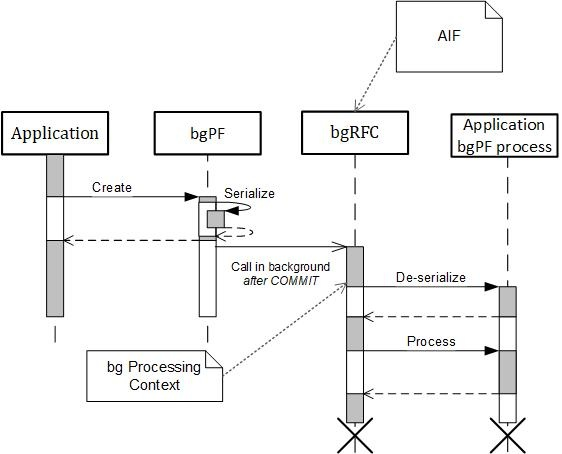
\includegraphics[height=8cm]{Bilder/bgPF_Schema.png}
 \caption[Funktionsweise des bgPF]{Funktionsweise des bgPF, Abgerufen von \cite{sap_bgpf_2023} am 17.07.2023.}
 \label{fig:iso_norm}
\end{figure}

Nachdem das Interface für das bgPF in der Anwendung als eigene Klasse mit der jeweiligen Logik, die ausgelagert werden soll, implementiert wurde, kann es verwendet werden. Die Anwendung ruft dann zur Laufzeit diese Klasse auf und erstellt synchron ein bgPF-Objekt. Innerhalb dieses Objekts wird die Klasse dann serialisiert und mit einem Methodenaufruf für die spätere Ausführung gespeichert. In der Endphase des Hauptprozesses wird dann mit einem bgRFC, also einem Funktionsaufruf, der im Hintergrund ausgeführt wird, die Ausführung ausgelöst. Der bgRFC wird dann in einer neuen ABAP Laufzeit als neuer Prozess gestartet. Hier wird die serialisierte Klasse wieder deserialisiert und die implementierte Logik ausgeführt. Nach dem Ausführen wird der Prozess wieder beendet. Falls nötig, können durch das Bereitstellen eines eigenen Verarbeitungskontexts von der aufrufenden Anwendung spezifische Verarbeitungsprioritäten festgelegt werden. Dies ist zwingend notwendig, wenn die Verarbeitungsreihenfolge genau eingehalten werden muss. Der voreingestellte Kontext wird standardä{\ss}ig von anderen Anwendungen gemeinsam verwendet. \footcite[Vgl.][]{sap_bgpf_2023}

Das Entkoppeln und asynchrone Ausführen gewisser Logik vom Hauptprozess bringt einige Vorteile mit sich: Zuerst wird die Robustheit und transaktionale Konsistenz des Hauptprozesses und somit auch die Konsistenz der Daten sichergestellt. Das bgPF bietet die Möglichkeit, diese Konsistenz zu gewährleisten, aber auch gleichzeitig relevantes Coding aus dem Hauptprozess auszulagern, was dessen Robustheit verbessert. Des Weiteren erscheint die Hauptanwendung für den Benutzer performanter, da gewisse Verarbeitungslogik in einer anderen Sitzung asynchron ausgeführt werden kann. Ein weiterer Vorteil ist die bessere Skalierbarkeit, wenn grö{\ss}ere Prozesse in kleinere Teile unterteilt werden, die verteilt über mehrere Laufzeitumgebungen asynchron ausgeführt werden können. Die Skalierung einer Anwendung kann mit dieser Technologie dann komplett vom SAP-System automatisiert werden. Diese Funktionalität des automatischen Skalierens befindet sich jedoch zum Zeitpunkt des Verfassens dieser Arbeit noch in der Entwicklung und ist noch nicht produktiv verfügbar. \footcite[Vgl.][]{sap_bgpf_2023}

\subsubsection{bgPF innerhalb von RAP}

Das bgPF kann auch innerhalb von RAP verwendet werden. Grundlegend besteht die Laufzeit eines RAP BOs aus einer Interaktions- und einer Speicherungsphase. In der Interaktionsphase werden über die Behaviours des BO dessen Daten ausgelesen oder verändert. Falls Änderungen an den Daten stattgefunden haben, werden diese jedoch nicht direkt auf der Datenbank persistiert, sondern zuerst in einem Puffer gespeichert. Nachdem alle Änderungen erfolgreich durchgeführt wurden, werden diese auf einmal in der Speicherungsphase auf die Datenbank geschrieben. Konkret wird die Methode des bgPF-Objekts, die das Speichern für die spätere asynchrone Ausführung übernimmt, in der zweiten Phase der Laufzeit des BOs aufgerufen und das Objekt somit auf der Datenbank gespeichert. \footcite[Vgl.][]{sap_bgpf_2023}

\section{Vergleich der Ansätze}

Im Folgenden sollen die in den vorherigen Kapiteln vorgestellten Ansätze miteinander verglichen werden. Hierfür werden die Kriterien Komplexität der Implementierung, also welchen Aufwand das Umsetzen der Technologie im Anwendungsfall verursacht, die Auswirkungen auf die Systemlandschaft, also ob zusätzliche Systemkomponenten benötigt werden und die Performance der einzelnen Ansätze im Bezug auf Ausführungsdauer und Rechenlast verglichen werden. Weitere Kriterien sind zusätzliche Kosten die eine Lösung eventuell verursacht, die Abwärtskompatibilität zu älteren Systemen und die Flexibilität der Technologien im Bezug auf Gestaltungsmöglichkeiten von Anwendungsszenarien und Integration mit anderen Technologien/ Frameworks. Abgeschlossen wird der Vergleich mit einer Betrachtung der Skalierbarkeit und Wartbarkeit der drei Umsetzungsmöglichkeiten.

\subsubsection{Komplexität der Implementierung}

Als erstes Kriterium wird die Komplexität der Implementierung der drei Technologien herangezogen. Genauer wird hier auf die Anzahl der zu erstellenden Artefakte, eine Beschreibung der Implementierungstätigkeiten und eine ungefähre Lines-of-Code Angabe betrachtet.

Die Komplexität von Workflows hängt von dem Geschäftsprozess ab, der abgebildet werden soll. Somit ist das Spektrum von einem sehr einfachen Workflow, der beispielsweise bei einem gewissen Ereignis einen Mitarbeiter per E-Mail benachrichtigt bis hin zu einem Workflow für einen komplexen Geschäftsprozess, wie einer Abwesenheitsmeldung, bei dem viele Schritte mit Genehmigungsprozessen nötig sind und der in viele Stellen im System hineingreift. Durch die freien Gestaltungsmöglichkeiten eines Workflows, einen Prozess aus beliebig vielen Schritten in beliebiger Konstellation zu modellieren sind Workflows in Produktivsystemen meistens sehr komplex. Hinzu kommt die weitgehenden Konfigurationsmöglichkeiten eines jeden Schrittes in einem Workflow und die Möglichkeit eigenes ABAP-Coding in einem Schritt auszuführen. Hierdurch kann die Komplexität nochmals stark steigen. Zudem können Workflows, wie oben angesprochen ereignisgesteuert gestartet werden und miteinander interagieren, wodurch komplexe Wechselwirkungen zusätzlich beachtet werden müssen. Somit lässt sich insgesamt sagen, dass Workflows zwar potenziell simpel sein können, jedoch in der Realität eher sehr komplex sind. (vgl. Anhang \ref{T_Workflows}, Z. 22-32)

Bei Business Events hängt die Komplexität vom der verwendeten Ansatz ab. Beispielsweise sind Standard Events von SAP sehr einfach, diese sind bereits im System vorhanden und müssen nur über eine Einstellung eingeschaltet werden. Dadurch ist das Event exponiert. Normalerweise werden die Events bereits von der SAP entwickelt und an die Kunden ausgeliefert. Wenn jedoch für eine spezielle Anforderung ein eigenes Event benötigt wird, kann auch ein Custom Event erstellt werden. Diese werden entweder RAP-basiert entwickelt, was einen nicht unerheblichen Aufwand darstellt und Erfahrung in der Entwicklung mit RAP voraussetzt. Die andere Option ist das Netweaver Event Enablement Add-On, womit man durch einen Low-Code-Ansatz ein Event einfach in kurzer Zeit konfigurieren kann. Insgesamt ist festzustellen, dass der Aufwand von wenigen Sekunden mit dem Aktivieren eines Standard Events bis hin zu mehreren Tagen mit einem selbst programmierten RAP-basiertem Event reicht. Auch die zu erstellenden Artefakte sind je nach verwendeter Technologie unterschiedlich. (vgl. Anhang \ref{T_Business-Events}, Z. 28-63)

Die Komplexität bei der Implementierung des bgPF beschränkt sich auf die Implementierung einer der zur Verfügung stehenden Interfaces. Ab hier übernimmt dann das Framework das Serialisieren und Weitergeben der Klasse an das bgRFC Framework, das dann für die asynchrone Ausführung zuständig ist. Die Komplexität des bgRFC Frameworks beschränkt sich für den Anwendungsprogrammierer, nachdem es initial beim Einrichten des Systems konfiguriert wurde auf wenige Zeilen Code, in denen die Einheit, die den Funktionsaufruf ausführt, aufgerufen wird. Hier ist die Komplexität jedoch wieder vom konkreten Anwendungsfall abhängig, da die Funktionen, die im Hintergrund ausgeführt werden sollen vom Entwickler selbst entwickelt werden müssen. Die Komplexität hängt also von der Geschäftsprozesslogik ab, die umgesetzt werden soll. Die Konfiguration des bgRFC Framework besteht im Groben aus dem Festlegen auf welchen Applikationsservern eine bgRFC Einheit ausgeführt werden soll und wie viele Ressourcen diese verbrauchen darf. Insgesamt kann man sagen, dass die Komplexität, abgesehen von der konkreten Anwendungslogik sich auf wenige Konfigurationen und Zeilen Code beschränkt und somit als mittelschwer eingestuft werden kann. (vgl. Anhang \ref{T_bgPF}, Z. 17-30)

\subsubsection{Auswirkungen auf die Systemlandschaft}

Die Auswirkungen auf die Systemlandschaft werden daran bemessen, ob für die Implementierung der jeweiligen Technologie zusätzliche Systemkomponenten, im Spezielleren das Einbinden von Cloud-Komponenten, notwendig sind.

Workflows sind in der sogenannten ''SAP-Basis'' enthalten. Die Systemkomponente ''SAP-Basis'' bildet die technische Grundlage eines SAP-Systems, indem sie Systemadministration, Datenbankmanagement, Kommunikation, Sicherheit und Performance-Optimierung gewährleistet und somit eine stabile und effiziente Plattform für die Ausführung der SAP-Anwendungen bereitstellt. Das hei{\ss}t, dass sie in jedem SAP-System als Grundfunktionalität verfügbar sind und somit mit dem initialen Lizenzkauf der Software benutzbar sind. Es müssten keine zusätzlichen Systemkomponenten integriert werden und Workflow sind sowohl in on-premise als auch in Cloud-Systemen verfügbar. Somit lässt sich zusammenfassen, dass Workflows keine Auswirkungen auf die Systemlandschaft haben. (vgl. Anhang \ref{T_Workflows}, Z. 33-40)

Das Verwenden von Business Events hat auf die Systemlandschaft definitiv mehrere Auswirkungen. Zum einen müssen die Prozesse des Unternehmens selbst angepasst werden, da man von synchronen batchorientierten Prozessen zu asynchronen Prozessen umsteigt. Zudem wird ein Event Broker oder Event Mesh (Netzwerk mehrerer Event Broker) als zusätzliche Systemkomponente benötigt, das den Austausch der Events regelt. Das SAP Event Mesh ist zudem eine Cloud-Komponente, was eine relevante Änderungen für reine on-premise Systemlandschaften darstellt. Es ist aber auch möglich einen Event Broker lokal zu betreiben, wenngleich dann die Vorteile der globalen Vernetzung mit Events verloren gehen. Zudem können mit SAP-Technologie auch Events anderer Hersteller, die dem Cloud Event Standard entsprechen verarbeitet werden, was für heterogene Systemlandschaften mit Systemen Lösungen mehrerer Hersteller ein gro{\ss}er Vorteil ist. (vgl. Anhang \ref{T_Business-Events}, Z. 64-108)

Auch das bgRFC Framework ist in der Systemkomponente SAP-Basis enthalten und ist somit bei jedem SAP System vorhanden und einsetzbar. Auch das Ausführen der remote function calls im Hintergrund passiert komplett lokal im System. Somit hat das bgRFC Framework an sich, wie Workflows keine Auswirkungen auf die Systemlandschaft. Das bgPF ist aber als darauf aufbauende Technologie zum heutigen Stand nur für Cloud Systeme verfügbar. Dies stellt aber eher einen Vorteil für Cloud Systeme als einen Nachteil für on-premise Systeme dar, weil die bgRFC Technologie nicht direkt in der Cloud verfügbar ist, sondern nur über den Umweg des bgPF. Zudem wird diese auch mit der Version von 2023 für on-premise Systeme verfügbar werden. Somit ergeben sich beim bgPF grundsätzlich keine Auswirkungen auf die Systemlandschaft, es muss lediglich zum jetztigen Zeitpunt bei Cloud Systemen das bgPF und bei on-premise Systemen der bgRFC benutzt werden.(vgl. Anhang \ref{T_bgPF}, Z. 31-49)

\subsubsection{Performance}

Die Performance der drei Lösungsansätze wird anhand der Rechenlast, die auf dem System durch das Ausführen des Prozesses erzeugt wird, der Ausführungsdauer und der Netzwerklast die dadurch entsteht gemessen.

Allgemein lässt sich sagen, dass der Performance-Aspekt bei Workflows in einer typischen Systemlandschaft kein Problem darstellt und auch bei sehr häufig stattfindenden Prozessen keine Leistungsgrenzen erreicht werden. Zudem werden Workflows, bedingt durch die Prozesse, die mit ihnen abgebildet werden, meist nicht auf einmal ausgeführt, sondern immer nur einzelne oder wenige Schritte. Diese Schritte erzeugen für sich keine nennenswerte Last auf dem System und sind meist sehr unterschiedlich. Der limitierende Faktor hingegen ist eher der Anwender, da in vielen Prozessen manuell Entscheidungen getroffen werden müssen oder der Benutzer aktiv Dinge tun muss, wodurch die Ausführung blockiert ist. Auch in dem Fall, dass viele Schritte eines Workflows hintereinander ausgeführt werden, bearbeitet das System alle Tätigkeiten im Hintergrund ohne den Anwender zu beeinflussen. Kommunikation über Systemgrenzen hinaus, die die Performance verschlechtern würde, ist zwar theoretisch möglich, aber in der Realität meist nicht notwendig und die Ausführung von Workflows findet beim Gro{\ss}teil der Geschäftsprozesse rein lokal statt. Somit sind Workflows insgesamt eine performante Technologie. (vgl. Anhang \ref{T_Workflows}, Z. 41-66)

Der Einsatz von Business Events ist für das Quellsystem der Events von erheblichem Vorteil, da durch den eventgesteuerten Ansatz die nachgelagerte Code-Ausführung gezielt ausgelöst werden kann und keine Last durch permanente API-Calls, um zu prüfen, ob das relevante Ereignis eingetreten ist, entsteht. Das ausschlaggebende Kriterium bei Business Events im Bezug auf die Performance sind die mitgeschickten Daten: Je mehr Daten bei einem Event mitgeschickt werden, desto grö{\ss}er wird es und desto mehr Last entsteht bei der Erzeugung und Weiterleitung. Hier gilt es, den Mittelweg zwischen der Menge an mitgeschickten Informationen und der Menge an API-Calls zu finden. Insgesamt dürfe das für den konkreten Anwendungsfall jedoch kein Problem darstellen, da kleine Benachrichtigungs-Events ausreichen, um eine asynchrone Code-Ausführung im Hintergrund anzusto{\ss}en. (vgl. Anhang \ref{T_Business-Events}, Z. 109-135)

Da mit dem bgPF bzw. bgRFC asynchrone Technologien betrachtet werden entsteht bei einem reinen Zeitaspekt aufgrund der Natur der Frameworks immer eine gewisse Verzögerung bei der Ausführung der speziellen Logik. Wie groß diese Verzögerung dann letztendlich ist, hängt wesentlich von den Konfigurationen des bgRFC ab, das auch beim bgPF für die Ausführung des Codes zuständig ist. Hier ist vor allem wichtig wie viele Ressourcen dem Framework zugewiesen werden, denn je mehr Rechenleistung zur Verfügung steht, desto schneller können die Funktionsaufrufe ausgeführt werden. Zudem kann konfiguriert werden wie viele Applikationsserver für die Ausführung solcher Hintergrundtätigkeiten genutzt werden. Hier sollten jedoch Wechselwirkungen mit anderen Systemkomponenten beachtet werden, da das restliche System beeinträchtigt werden kann, wenn für alle anderen Prozesse nicht mehr genug Leistung zur Verfügung steht. Somit lässt sich zusammenfassen, dass aufgrund der Ausführung im Hintergrund zwar immer eine gewisse Verzögerung in Kauf genommen werden muss, diese aber durch die Zuteilung von mehr oder weniger Ressourcen steuerbar ist. (vgl. Anhang \ref{T_bgPF}, Z. 50-61)

\subsubsection{Kosten}

Zunächst wird die monetäre Seite der drei Technologien betrachtet. Es soll die Frage beantwortet werden, ob durch die drei Technologien zusätzliche Lizenzkosten, laufende Kosten durch Abonnements und Kosten für Netzwerk-Traffic entstehen. 

Da die Workflows in der SAP-Basis mit jedem System enthalten sind, entstehen für den Kunden keine weiteren Kosten durch die Implementierung dieser Technologie. (vgl. Anhang \ref{T_Workflows}, Z. 67-72)

Die Implementierung von Business Events verursacht Kosten. Zum einen durch das Betreiben eines Brokers, wie \zB dem SAP Event Mesh. Kleinere Broker wie dieser, die vor Allem auf kleinere Notification-Events ausgelegt sind, werden gemietet und nach dem Benutzungsvolumen bezahlt. Hier liegen die Kosten, wenn nur einzlene Anwendungsfälle oder Bereiche abgebildet werden im dreistelligen Bereich pro Monat. Soll jedoch die gesamte Unternehmensarichtektur mit Events gesteuert werden, müssen umfangreichere Technologien zum Einsatz kommen, bei denen die Kosten schnell im sechsstelligen Bereich liegen. Hier ist der relevante Faktor die Betrachtung des Break-even-Punkts, ab dem man Geld spart, da die Infrastruktur vorhanden ist und Skaleneffekte eintreten. Ab welcher Anzahl an Events diese Technologie günstiger ist, muss im Einzelfall betrachtet werden. Im konkreten Anwendungsfall sollte das nicht gegen Business Events als Lösungsansatz sprechen, da hier nur ein spezieller Anwendungsfall mit kleinen Events betrachtet wird, der auch mit dem SAP Event Mesh abgebildet werden kann. (vgl. Anhang \ref{T_Business-Events}, Z. 136-163)

Bei dem bgPF fällt die Bewertung des Kostenfaktors, ähnlich wie bei Workflows, sehr kurz aus, da auch hier die relevante Technologie bereits in der SAP Basiskomponente enthalten ist und somit in jedem SAP System benutzbar ist. Hier muss zwar der Vollständigkeit halber angemerkt werden, dass man sich in Cloud Systemen für das bgPF und in on-premise Systemen für das bgRFC Framework entscheiden muss, was aber keine Einschränkungen bedeutet, da beide dieselbe Funktionalität bereitstellen. Auch wenn das Cloud System laufende Kosten verursacht, so entstehen diese aufgrund des Gesamtsystems und nicht aufgrund der Verwendung des bgPF. Somit entstehen hier keine zusätzlichen Kosten für den Anwender. (vgl. Anhang \ref{T_bgPF}, Z. 62-65)

\subsubsection{Flexibilität}

Beim Kriterium der Flexibilität soll die spätere Anpassbarkeit der Lösungsansätze, die Gestaltungsmöglichkeiten die sie bei spezielleren Anforderungen bieten und die Integrationsmöglichkeiten zu anderen Technologien betrachtet werden.

Bei der Flexibilität von Workflows muss zwischen klassischen und flexiblen Workflows unterschieden werden. Bei der Betrachtung der Gestaltungsmöglichkeiten bei speziellen Anforderungen verhalten sich beide Varianten gleich, die Vorlagen, die hier von SAP an Kunden ausgeliefert werden, sind nochmals an die konkreten Bedürfnisse und Geschäftsprozesse anpassbar. Im Bezug auf die spätere Anpassbarkeit sind flexible Workflows im Vorteil, da hier Fehlerkorrekturen im Gegensatz zu klassischen Workflows automatisch im Kundensystem übernommen werden, sobald diese von der SAP veröffentlicht wurden. Bei klassischen Workflows müssen diese noch aktiv vom Kunden umgesetzt werden. Jedoch sind flexible Workflows nur für Cloud-Produkte verfügbar. Die Integrationsmöglichkeiten mit anderen Technologien sind für Workflows auch sehr umfangreich, da auf diese als Teil der SAP-Basis von allen anderen Softwarekomponenten aus zugegriffen werden kann. Insgesamt sind Workflows sehr flexibel, da der Kunde nicht an die Vorlagen der SAP gebunden ist und durch das Ausführen von eigenem ABAP-Coding weitgehende Freiheiten hat. (vgl. Anhang \ref{T_Workflows}, Z. 73-115)

Die Flexibilität von Business Events hängt stark von der verwendeten Technologie ab. Auf der einen Seite gibt es Standard-Events, die sehr unflexibel sind, auf der anderen Seite sind Custom Events mit dem Netweaver Event-Enablement Add-On sehr flexibel und schnell anpassbar. Durch die Möglichkeit ein eigenes Event mit RAP zu programmieren erhält der Entwickler fast unbegrenzte Freiheiten, solange man sich im Cloud Events Standard bewegt. Events lassen sich auch untereinander mit anderen Events kombinieren. Diese können \zB beim Passieren des Event Brokers verändert werden oder in anderen Systemkomponenten gewisse Logik auslösen. Somit sind Business Events insgesamt im Bezug auf ihre spätere Anpassbarkeit und ihre Integrationsmöglichkeiten mit anderen Technologien sehr flexibel. (vgl. Anhang \ref{T_Business-Events}, Z. 164-186)

Aufgrund der Funktionsweise des bgPF bzw. bgRFC Frameworks lassen sich die ersten beiden Subkriterien der Flexibilität kurz ausführen. Die Aufgabe der Frameworks ist es lediglich, beliebigen Code asynchron im Hintergrund auszuführen. Die Anpassbarkeit dieses Codes und die Möglichkeiten bei speziellen Anforderungen sind somit auf der rein funktionalen Ebene unabhängig vom ausführenden Framework an sich. Somit kann hier resümiert werden, dass die Umsetzbarkeit spezieller Anforderungen und Anpassbarkeit lediglich durch die Möglichkeiten, die ABAP als Programmiersprache zur Verfügung stellt, begrenzt wird und somit kein Problem darstellen sollte. Die Integrationsmöglichkeiten mit anderen Technologien sind genauso wie bei Workflows sehr umfangreich, da auch auf den bgRFC als Teil der SAP-Basis von allen anderen Komponenten aus zugegriffen werden kann und das bgPF in der Cloud auch durch das Implementieren eines Interfaces überall einsetzbar ist. (vgl. Anhang \ref{T_bgPF}, Z. 66-79)

\subsubsection{Skalierbarkeit}

Die Skalierbarkeit der Komponenten beschreibt ihre Fähigkeit bei wachendem Nutzungsvolumen und Datenlast effizient zu wachsen und die Leistung beibehalten. Genauer wird hier die Aufteilbarkeit der Technologien auf mehrere Prozesse und das Vorhandensein von Frameworks, die die Skalierung automatisch abwickeln herangezogen.

Workflows sind an sich gro{\ss}e zusammenhängende Prozesse, die aufgrund der sequentiellen Reihenfolge der einzelnen Schritte nicht unterteilt und \zB parallel ausgeführt werden können. Somit skalieren Workflows nur linear, die Menge an beanspruchten Ressourcen steigt proportional zur Anzahl der laufenden Prozesse. (vgl. Anhang \ref{T_Workflows}, Z. 116-127)

Das Thema Skalierbarkeit ist eine der gro{\ss}en Stärken von Business Events. Event Broker sind darauf ausgelegt bis hin zu mehreren Milliarden von Events pro Tag zu verarbeiten und weiterzuleiten. Bei dieser Technologie erreichen als erstes das Back-End-System, von dem aus die Events losgeschickt werden oder das System, das die Events letztendlich empfängt ein Limit. Aber auch dieses Limit wird erst sehr spät erreicht, da die Technologie allgemein auf starke Skalierung ausgelegt ist. (vgl. Anhang \ref{T_Business-Events}, Z. 187-193)

Beim Kriterium der Skalierbarkeit hat das bgPF noch einige Defizite gegenüber dem bgRFC. Hier ist die Ausführung in lediglich einem Applikationsserver möglich, was die Ressourcenzuteilung je nach Aufgaben und den Last-Ausgleich zwischen den verschiedenen Applikationsservern erschwert. Wenn ein on-premise System vorhanden ist, ist es möglich verschiedene Applikationsserver für die Ausführung von Logik im Hintergrund zu benutzen und diesen auch unterschiedlich viele Ressourcen einzuräumen. Somit ist hier der bgRFC im Vorteil gegenüber dem bgPF, was zum jetzigen Entwicklungszeitpunkt noch diese Defizite im Bezug auf die Skalierbarkeit aufweist. (vgl. Anhang \ref{T_bgPF}, Z. 80-92)

\subsubsection{Wartbarkeit}

Software wird als leicht wartbar bezeichnet, wenn sie leicht verändert, erweitert, repariert und aktualisiert zu werden, um Fehler zu beheben oder neue Anforderungen zu erfüllen. Dieses Kriterium wird anhand der Analysemöglichkeiten, die für eine Technologie zur Verfügung stehen und ob notwendige Anpassungen an einer Stelle oder über mehrere Systeme verteilt erfolgen müssen, bewertet.

Workflows werden im SAP-System zentral an einer Stelle erstellt, konfiguriert und verwaltet. Von dieser Stelle kann auch zentral das Debugging stattfinden, auch wenn andere Systemkomponenten beeinflusst werden. Somit kann die Wartung als relativ einfach beschrieben werden. 

Die Wartbarkeit von Business Events wird ma{\ss}geblich davon beeinflusst, inwieweit die Grundsätze der eventgesteuerten Architektur bei der Implementierung eingehalten wurden. Dann kann die gesamte Wartung nur an der Eventquelle geschehen, da die Events unabhängig von ihrem Konsumenten konstruiert sind. Realistisch ist der Wartungsaufwand und die Komplexität jedoch etwas höher, da oft Konsumenten schon im Voraus aus Effizienzgründen Annahmen über die Gestalt der Events treffen. Somit muss die Wartung dann neben dem Quell-System auch beim Konsumenten und dem Event Broker erfolgen. Auch die Art der Events ist entscheidend, da kleinere Notification Events grundsätzlich einfacher zu warten sind als gro{\ss}e Daten Events. Insgesamt sind Business Events jedoch gut wartbar. (vgl. Anhang \ref{T_Business-Events}, Z. 194-212)

Da das bgPF durch das Implementieren eines Interfaces benutzt werden kann, ist hier die gesamte Wartbarkeit für die Anwendungsfälle direkt im Code oder über den ABAP Debugger möglich und somit sehr einfach. Für die darunterliegende Technologie gibt es einen Transaktionscode von dem aus das bgRFC Framework komplett konfiguriert werden kann. Somit kann die Wartbarkeit als relativ einfach eingeordnet werden. (vgl. Anhang \ref{T_bgPF}, Z. 93-100)

\subsubsection{Abwärtskompatibilität}

Zuletzt wird noch die Abwärtskompatibilität der Ansätze betrachtet. 

Klassische Workflows sind keine neue Technologie mehr und funktionieren in allen gängigen (auch älteren) SAP-Systemen. Auf flexible Workflows trifft das jedoch nicht zu, da diese für die Cloud entwickelt wurden und eine neuere Technologie sind. Bei klassischen Workflows wurde in neueren Versionen lediglich die Benutzeroberfläche angepasst, die Funktionalität ist gleich geblieben. Somit können Workflows, die in neueren Versionen entwickelt wurden problemlos in ältere Systeme kopiert werden. Zusammenfassend eigenen sich Workflows sehr gut, wenn Abwärtskompatibilität ein wichtiges Kriterium ist.

Die Abwärtskompatibilität wird auch im Wesentlichen von der verwendeten Technologie bestimmt. Sollen Standard Events zum Einsatz kommen, muss das S/4 Back-End-System immer auf der aktuellsten Version sein, da ältere Versionen die neuen Features nicht unterstützen. Genau für ältere Systeme gibt es das Event Enablement Add-On, was dafür ausgelegt ist, auch noch mit alten SAP ECC Systemen zu arbeiten. Somit sind Business Events zumindest teilweise abwärtskompatibel.(vgl. Anhang \ref{T_Business-Events}, Z. 213-223)

Das bgPF ist noch eine sehr neue Technologie, die auch im Moment noch weiterentwickelt wird. Somit ist hier eine Abwärtskompatibilität nicht wirklich gegeben. Dieser Faktor an sich ist jedoch unerheblich, da das Framework sowieso nur in der Cloud verfügbar ist und die Systeme der Kunden hier ohne ihr Zutun immer die neueste Version haben. In einer on-premise Landschaft stellt die Abwärtskompatibilität kein Problem dar, da die bgRFC Technologie schon seit dem Release 701, also schon seit 2005 existiert und somit mit dem Großteil der produktiven Systeme kompatible sein sollte. Insgesamt ist somit im on-premise Umfeld eine sehr gute Abwärtskompatibilität gegeben, in der Cloud jedoch nicht. (vgl. Anhang \ref{T_bgPF}, Z. 101-112)

\section{Entscheidungsmatrix}

Hier soll eine Entscheidungsmatrix entwickelt werden, welchen Lösungsansatz man in Abhängigkeit von mehreren Faktoren am besten verwenden soll. \newline

% mögliche Vergleichskriterien:

% - Komplexität der Implementierung (Ranking: Workflow > Business Events > bgPF) -> Lines of Code, Artefakte \newline
% - Systemlandschaft (Cloudkomponente (Datenschutz) EventMesh von BTP bei Business Events nötig, bgPF/ Workflows brauchen das nicht) \newline
% - Performance (Rechenlast, Zeit) (BE nicht so gut, weil Kommunikation über Web zu Cloud über HTTP, bgPF <-> Workflows nehmen sich nicht viel) \newline
% - Kosten (Vorteil Workflows: Release (Abwärts-) Kompatibilität zu ECC (gibts schon immer), Drängen von Kunden auf Funktionsverfügbarkeit in alten Systemen) (BE: Lizenzkosten für BTP Komponente, Netzwerklast durch HTTP Kommunikation bei Kunde) \newline
% - Flexibilität (Workflows sehr flexibel, viele Anbindungen, sehr gute Integration zu zB. Emails) (Beiden anderen Techniken eher low level Code, wenig Anbindungen an andere Frameworks) \newline
% - Skalierbarkeit (Workflows (nicht aufteilbar), BE überhaupt nicht) (bgPF Autoskalierbar, -> siehe Praxiskapitel) \newline
% - Wartbarkeit (Workflows extrem gut wartbar -> komplett auf ABAP-Instanz debuggbar/ nachvollziehbar) (bgPF ähnlich) (BE schlechte Wartbarkeit, da über viele Systeme, Frameworks, intransparente Analysemöglichkeiten)